% \iffalse
\let\negmedspace\undefined
\let\negthickspace\undefined
\documentclass[journal,12pt,twocolumn]{IEEEtran}
\usepackage{cite}
\usepackage{amsmath,amssymb,amsfonts,amsthm}
\usepackage{algorithmic}
\usepackage{graphicx}
\usepackage{textcomp}
\usepackage{xcolor}
\usepackage{txfonts}
\usepackage{listings}
\usepackage{enumitem}
\usepackage{mathtools}
\usepackage{gensymb}
\usepackage{comment}
\usepackage[breaklinks=true]{hyperref}
\usepackage{tkz-euclide} 
\usepackage{listings}
\usepackage{gvv}                                        
\def\inputGnumericTable{}                                 
\usepackage[latin1]{inputenc}                                
\usepackage{color}                                            
\usepackage{array}                                            
\usepackage{longtable}                                       
\usepackage{calc}                                             
\usepackage{multirow}                                         
\usepackage{hhline}                                           
\usepackage{ifthen}                                           
\usepackage{lscape}

\newtheorem{theorem}{Theorem}[section]
\newtheorem{problem}{Problem}
\newtheorem{proposition}{Proposition}[section]
\newtheorem{lemma}{Lemma}[section]
\newtheorem{corollary}[theorem]{Corollary}
\newtheorem{example}{Example}[section]
\newtheorem{definition}[problem]{Definition}
\newcommand{\BEQA}{\begin{eqnarray}}
\newcommand{\EEQA}{\end{eqnarray}}
\newcommand{\define}{\stackrel{\triangle}{=}}
\theoremstyle{remark}
\newtheorem{rem}{Remark}
\begin{document}



\bibliographystyle{IEEEtran}
\vspace{3cm}

\title{NCERT 11.9.5 26Q}
\author{EE23BTECH11015 - DHANUSH V NAYAK$^{*}$% <-this % stops a space
}
\maketitle
\newpage
\bigskip

\renewcommand{\thefigure}{\theenumi}
\renewcommand{\thetable}{\theenumi}

\bibliographystyle{IEEEtran}
\textbf{Question:} Show that
\begin{equation}
    \frac{1\times2^2 + 2\times3^2 + \dots + n\times(n+1)^2}{1^2\times2 + 2^2\times3 +\dots + n^2\times(n+1)}  = \frac{3n+5}{3n+1}\notag
\end{equation}\\
\textbf{Solution:}\\
\begin{enumerate}[label=\alph*)]
\item Consider the Numerator of the LHS part:
\begin{equation}
    1\times2^2 + 2\times3^2 + \dots + n\times(n+1)^2 = \sum_{k=1}^n k(k+1)^2 
\end{equation}
Now,
\begin{align}
    \sum_{k=1}^n k(k+1)^2 &= \sum_{k=1}^n k^3+2k^2+k\\
                          &=  \sum_{k=1}^n k^3 + \sum_{k=1}^n 2k^2 + \sum_{k=1}^n k\\
                          &=  \sum_{k=1}^n k^3 + 2\sum_{k=1}^n k^2 + \sum_{k=1}^n k\\
                          &= \left(\frac{n(n+1)}{2}\right)^{\scriptstyle 2} + 2\cdot \frac{n(n+1)(2n+1)}{6}+\\  &+\frac{n(n+1)}{2}\notag \\
                          &= \frac{n(n+1)}{2}\left[\frac{n(n+1)}{2} + \frac{2}{3}(2n+1) + 1\right]\\
                          &= \frac{n(n+1)}{2}\left[\frac{3n^2 + 11n +10}{6}\right]\\
                          &= \frac{n(n+1)}{12}\left[3n^2 + 6n + 5n + 10\right]\\
                          &= \frac{n(n+1)}{12}\left[3n(n+2)+5(n+2)\right]\\
                          &= \frac{n(n+1)(n+2)(3n+5)}{12}
\end{align}
Therefore,
\begin{equation}
   1\times2^2 + 2\times3^2 + \dots + n\times(n+1)^2 = \frac{n(n+1)(n+2)(3n+5)}{12}   \\
\end{equation}
\begin{align}
    \frac{n(n+1)(n+2)(3n+5)}{12}\cdot u[n] = x[n]
\end{align}
\begin{figure}[h]
        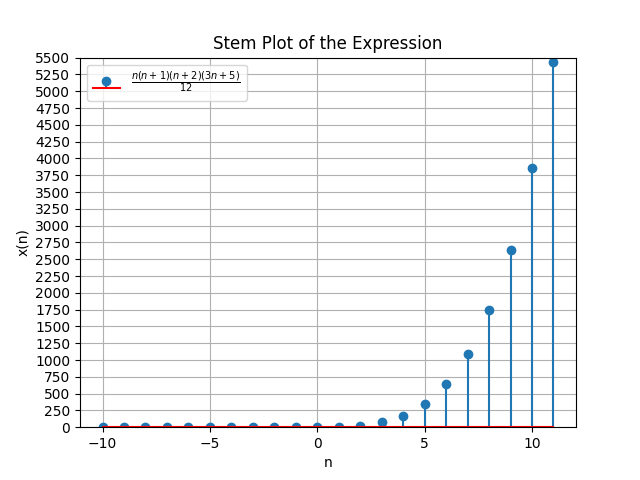
\includegraphics[width=\columnwidth]{Figure_1.png}
        \caption{Stem Plot of x[n]}
    \end{figure}
    
Derivation of z-transform of numerator :
\begin{align}
    x[n] &= \frac{n(n+1)(n+2)(3n+5)}{12}\cdot u[n]\\
         &= \frac{3n^4 + 14n^3 + 21n^2 + 10n}{12}\cdot u[n]\
\end{align}
\begin{equation}
    X(z) = \sum_{n=-\infty}^\infty x[n]z^{-n}
\end{equation}
Z-Transform is calculated as:
\begin{equation}
    X(z) = \sum_{n=-\infty}^\infty x[n]\cdot z^{-n}
\end{equation}
\begin{align}
    X(z) &= \sum_{n=-\infty}^\infty\frac{3n^4 + 14n^3 + 21^2 + 10n}{12}
\end{align}
\begin{align}\label{eq:3}
    12X(z) &= \sum_{n=0}^\infty 3n^4z^{-n} +  \sum_{n=0}^\infty 14n^3z^{-n} \\ &+  \sum_{n=0}^\infty 21n^2 z^{-n} +\sum_{n=0}^\infty 10n\hspace{3pt} z^{-n}\notag
\end{align}
\text{Let $U(z)$ be z transform of $u[n]$.}
    \begin{align}
U(z) &= \sum_{n=0}^{\infty} u[n]\cdot z^{-n} \\
     &= \sum_{n=0}^{\infty} (1) \cdot z^{-n} \\
     &= 1 + z^{-1} + z^{-2} + \ldots \\
     &= \frac{1}{1 - z^{-1}} 
\end{align}

By the differentiation property:\\
\begin{align}
x[n] &\stackrel{\mathcal{Z}}{\longleftrightarrow} X(z)\\
n^k x[n] &\stackrel{\mathcal{Z}}{\longleftrightarrow} (-z)^k \frac{d^kX(z)}{dz^k}\\
n^k u[n] &\stackrel{\mathcal{Z}}{\longleftrightarrow} (-z)^k \frac{d^kU(z)}{dz^k} \label{eq:24}
\end{align}

\text{For the Z-transform of n \cdot u[n],}\\

\text{ substituting } k=1 \text{ in Equation \eqref{eq:24}:}
\begin{align}
    n \cdot u[n] &\stackrel{\mathcal{Z}}{\longleftrightarrow} -z \frac{dX(z)}{dz}\\
    \frac{dX(z)}{dz} &= -\frac{1}{(z - 1)^2}, \\
    X_1(z) &= \frac{z^{-1}}{(1-z^{-1})^2}.
\end{align}
\text{Substituting } k=2,3,4:
\begin{align}
     X_2(z) &= \frac{z^{-1}(z^{-1}+1)}{(1-z^{-1})^3}\\
     X_3(z) &= \frac{z^{-1}(1+4z^{-1}+z^{-2})}{(1-z^{-1})^4}\\
    X_4(z) &= \frac{z^{-1}(1+11z^{-1}+11z^{-2}+z^{-3})}{(1-z^{-1})^5} 
\end{align}

The Region of Convergence (ROC) is defined as the set of points in the complex plane for which the Z-transform summation converges, i.e., doesn't blow up in magnitude to infinity:
The Region of Convergence (ROC) is defined as:
\begin{equation}\label{eq:roc_definition}
    \text{ROC} = \left\{ z : \left| \sum_{n=-\infty}^{\infty} x[n]z^{-n} \right| < \infty \right\}
\end{equation}

Equation \eqref{eq:roc_definition} expresses the set of points in the complex plane for which the Z-transform summation converges.

The Z-transform of the unit step signal \(u[n]\) is given by:
\begin{equation}\label{eq:z_transform}
    U(z) = \sum_{n=-\infty}^{\infty} u[n] z^{-n}
\end{equation}

Since \(u[n] = 1\) for \(n \geq 0\) and \(u[n] = 0\) for \(n < 0\), the summation simplifies to:
\begin{equation}\label{eq:z_transform_simplified}
    U(z) = \sum_{n=0}^{\infty} z^{-n}
\end{equation}
\begin{equation}
    \text{ROC} = \left\{ z : \left| \sum_{n=0}^{\infty} z^{-n} \right| < \infty \right\}
\end{equation}
This is an infinite GP. And it converges only if $|r|<1$ where r is the common ratio.And here , $|r|=|z^{-1}|$ Therefore,
the Region of Convergence (ROC) for this Z-transform is:
\begin{equation}\label{eq:roc}
    \text{ROC: } |z| > 1
\end{equation}
In the differentiation property, ROC does not change:\\
\begin{align}
x[n] &\stackrel{\mathcal{Z}}{\longleftrightarrow} X(z),\hspace{4pt} ROC = R\\
n^k x[n] &\stackrel{\mathcal{Z}}{\longleftrightarrow} (-z)^k \frac{d^kX(z)}{dz^k},\hspace{4pt} ROC = R 
\end{align}
Therefore,
\begin{align}
    X_1(z) &= \frac{z^{-1}}{(1-z^{-1})^2} , \hspace{4pt} ROC=|z|>1\\
    X_2(z) &= \frac{z^{-1}(z^{-1}+1)}{(1-z^{-1})^3} , \hspace{4pt} ROC=|z|>1\\
    X_3(z) &= \frac{z^{-1}(1+4z^{-1}+z^{-2})}{(1-z^{-1})^4}, \hspace{4pt} ROC=|z|>1\\
    X_4(z) &= \frac{z^{-1}(1+11z^{-1}+11z^{-2}+z^{-3})}{(1-z^{-1})^5}, \hspace{4pt} ROC=|z|>1
\end{align}
Equation\eqref{eq:3} can be now written as:
\begin{align}
    X(z) &=\frac{1}{12}(3X_4(z) + 14X_3(z) + 21X_2(z) + 10X_1(z)) \\
         &= \frac{3}{12}\left(\frac{z^{-1}(1+11z^{-1}+11z^{-2}+z^{-3})}{(1-z^{-1})^5}\right)\\ &+ \frac{14}{12}\left(\frac{z^{-1}(1+4z^{-1}+z^{-2})}{(1-z^{-1})^4}\right) 
         + \frac{21}{12}\left(\frac{z^{-1}(z^{-1}+1)}{(1-z^{-1})^3}\right)\notag \\ &+ \frac{10}{12}\left(\frac{z^{-1}}{(1-z^{-1})^2}.\right)\notag \\
         &= \frac{2(z^{-2}+2z^{-1})}{(1-z^{-1})^5}
\end{align}

Consider the linear combination of two signals in the time domain:
\begin{align}
    a_1 x_1(n) + a_2 x_2(n) &= a_1 X_1(z) + a_2 X_2(z) \label{eq:combined_signal}\\
    \text{ROC} &= \text{ROC}_1 \cap \text{ROC}_2 \label{eq:roc_intersection}
\end{align}
Therefore, ROC of equation\eqref{eq:3} is the intersection of the ROC of each signal. Every signal has ROC $|z|>1$. So,
\begin{align}
    \text{ROC of $X(z)$} \text{\hspace{3pt}is\hspace{3pt}} |z|>1
\end{align}
  \item Consider the Denominator of the RHS part:
\begin{equation}
    1^2\times2 + 2^2\times3 +\dots + n^2\times(n+1) = \sum_{k=1}^n k^2(k+1)
\end{equation}
Now,\\
\begin{align}
     \sum_{k=1}^n k^2(k+1) &= \sum_{k=1}^n k^3+k^2\\
                           &=  \sum_{k=1}^n k^3 + \sum_{k=1}^n k^2\\
                           &=  \left(\frac{n(n+1)}{2}\right)^{\scriptstyle 2}+\frac{n(n+1)(2n+1)}{6}\\ 
                           &= \frac{n(n+1)}{2}\left[\frac{n(n+1)}{2} +\frac{2n+1}{3}\right]\\
                           &= \frac{n(n+1)}{2}\left[\frac{3n^2+7n+2}{6}\right]\\
                           &= \frac{n(n+1)}{12}\left[3n^2+6n + n+2\right]\\
                           &= \frac{n(n+1)}{12}\left[3n(n+2)+(n+2)\right]\\
                           &= \frac{n(n+1)(n+2)(3n+1)}{12}
\end{align}
\begin{align}
    \frac{n(n+1)(n+2)(3n+1)}{12}\cdot u[n] &= y[n]
\end{align}
\begin{figure}[h]
        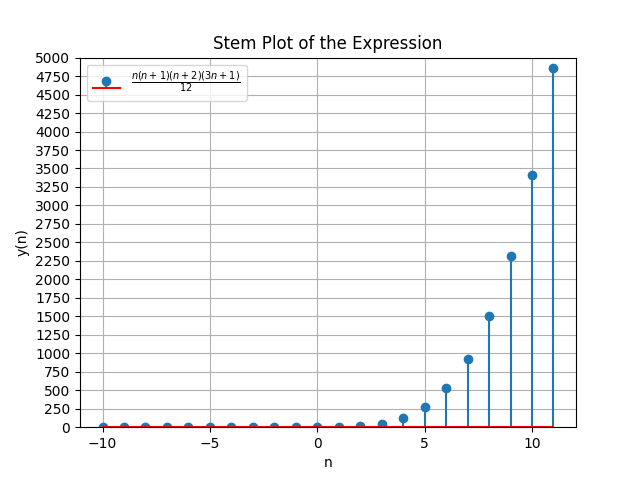
\includegraphics[width=\columnwidth]{Figure_2.png}
        \caption{Stem Plot of y[n]}
    \end{figure}
\vspace{1cm}

The Ncert question result is proved,
\begin{align}
     \dfrac{ \sum_{k=1}^n k(k+1)^2 }{\sum_{k=1}^n k^2(k+1)} &= \dfrac{\frac{n(n+1)(n+2)(3n+5)}{12}}{\frac{n(n+1)(n+2)(3n+1)}{12}}\\
                                                            &= \frac{3n+5}{3n+1}
\end{align}

Derivation of z-transform of the denominator:
\begin{align}
    y[n] &= \frac{n(n+1)(n+2)(3n+1)}{12}\cdot u[n]\\
         &= \frac{3n^4 + 10n^3 + 9n^2 + 2n}{12}\cdot u[n]\
\end{align}

\begin{equation}
    Y(z) = \sum_{n=-\infty}^\infty y[n]\cdot z^{-n}
\end{equation}
Z-Transform is calculated as:
\begin{align}\label{eq:9}
    Y(z) &= \sum_{n=-\infty}^\infty\frac{3n^4 + 10n^3 + 9n^2 + 2n}{12}\\
    12Y(z) &= \sum_{n=0}^\infty 3n^4z^{-n} +  \sum_{n=0}^\infty 10n^3z^{-n}\\ &+  \sum_{n=0}^\infty 9n^2 z^{-n} +\sum_{n=0}^\infty 2n\hspace{3pt}z^{-n}\notag
\end{align}
We can say that $Y_i$ denote the z-transform of $n^{i}$ which will be same as respective $X_i$.
\begin{align}\label{eq:61}
    X_i=Y_i
\end{align}
Equation\eqref{eq:9} can be now written as:
\begin{align}
    Y(z) &=\frac{1}{12}(3Y_4(z) + 10Y_3(z) + 9Y_2(z) + 2Y_1(z)) \\
         &= \frac{3}{12}\left(\frac{z^{-1}(1+11z^{-1}+11z^{-2}+z^{-3})}{(1-z^{-1})^5}\right)\\ &+ \frac{10}{12}\left(\frac{z^{-1}(1+4z^{-1}+z^{-2})}{(1-z^{-1})^4}\right) 
         + \frac{9}{12}\left(\frac{z^{-1}(z^{-1}+1)}{(1-z^{-1})^3}\right)\notag \\ &+ \frac{2}{12}\left(\frac{z^{-1}}{(1-z^{-1})^2}.\right)\notag \\
         &= \frac{2(z^{-1}+2z^{-2})}{(1-z^{-1})^5}
\end{align}
\(Y(z)\) is a linear combination of \(Y_i(z)\) for \(i=1,2,3,4\):
\begin{align}
    Y(z) &= a_1 Y_1(z) + a_2 Y_2(z) + a_3 Y_3(z) + a_4 Y_4(z) \label{eq:linear_combination_Y} \\
    \text{ROC}_{Y} &= \text{ROC}_{1} \cap \text{ROC}_{2} \cap \text{ROC}_{3} \cap \text{ROC}_{4} \label{eq:roc_Y}
\end{align}
By equation\eqref{eq:61} we can say that $Y_i$ also has same ROC as respective $X_i$. Therefore,\\
\begin{align}
    \text{ROC of $Y(z)$} : |z|>1
\end{align}
\end{enumerate}
\end{document}
